\documentclass[margin=2mm]{standalone}
\usepackage{tikz}
\usetikzlibrary{calc}
\usetikzlibrary{patterns}
\usetikzlibrary{decorations.text}
\usetikzlibrary{decorations.pathmorphing}
\usetikzlibrary{decorations.markings}

\begin{document}
% For every picture that defines or uses external nodes, you'll have to
% apply the 'remember picture' style. To avoid some typing, we'll apply
% the style to all pictures.
\tikzstyle{every picture}+=[remember picture]
\tikzstyle{na} = [baseline=-.5ex]

\begin{tikzpicture}%[show background grid]% every node/.style={draw,outer sep=0pt,thick}]

\tikzstyle{ground}=[fill, pattern=north west lines, draw=none]
\newcommand{\CoG}[1]{%
    \draw (#1) circle[radius=7pt, black, line width = 1pt];%
    \filldraw[black, line width=0.1pt] (#1) ++( 9pt,   0) -- ++(-18pt,     0);%
    \filldraw[black, line width=0.1pt] (#1) ++(   0, 9pt) -- ++(    0, -18pt);%
    \filldraw[black, line width=0.1pt] (#1) -- ++( 5pt,0) arc (  0:90 :5pt) -- cycle;%
    \filldraw[black, line width=0.1pt] (#1) -- ++(-5pt,0) arc (180:270:5pt) -- cycle;%
    %\node[anno-ptr, xshift=5pt, yshift=-5pt, anchor = north west] at
    %(#1) {CoM};%
}
\newcommand{\CoGsmall}[1]{%
    \draw (#1) circle[radius=4pt, black, line width = 1pt];%
    \filldraw[black, line width=0.1pt] (#1) ++( 5pt,   0) -- ++(-10pt,     0);%
    \filldraw[black, line width=0.1pt] (#1) ++(   0, 5pt) -- ++(    0, -10pt);%
    \filldraw[black, line width=0.1pt] (#1) -- ++( 3pt,0) arc (  0:90 :3pt) -- cycle;%
    \filldraw[black, line width=0.1pt] (#1) -- ++(-3pt,0) arc (180:270:3pt) -- cycle;%
    %\node[anno-ptr, xshift=5pt, yshift=-5pt, anchor = north west] at
    %(#1) {CoM};%
}

% Put the graphic inside a node. This makes it easy to place the
% graphic and to draw on top of it.
% The above right option is used to place the lower left corner
% of the image at the (0,0) coordinate.
\node [inner sep=0pt,above right] {
    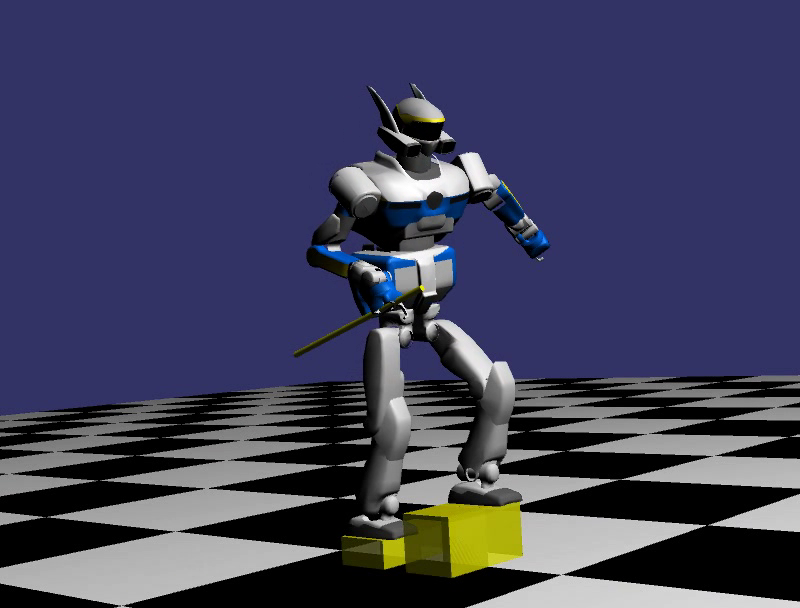
\includegraphics[width=1.0\linewidth]{../hrp2_free_waist_dynamic.png}
};

% coordinate system
\def\cosxaxis{1.0}
\def\sinxaxis{0.0}
\def\cosyaxis{ 0.866025403784}
\def\sinyaxis{ 0.5}
\def\coszaxis{0.0}
\def\sinzaxis{1.0}

% define origin
%\coordinate (origin) at (0.0, 0.0);

% define origin of world
%\coordinate (cos_ori) at (0.5, 0.5);
%\fill[magenta] (cos_ori) circle (2pt); % show origin

%\def\ax_length{1.0}
%\path (cos_ori) ++ ( \ax_length * \cosxaxis, \ax_length * \sinxaxis) coordinate (cos_x);
%\def\ax_length{0.7}
%\path (cos_ori) ++ ( \ax_length * \cosyaxis, \ax_length * \sinyaxis) coordinate (cos_y);
%\def\ax_length{1.0}
%\path (cos_ori) ++ ( \ax_length * \coszaxis, \ax_length * \sinzaxis) coordinate (cos_z);

%\draw [->,thick, teal!20] (cos_ori) -- (cos_x);
%\draw [->,thick, teal!20] (cos_ori) -- (cos_y);
%\draw [->,thick, teal!20] (cos_ori) -- (cos_z);

%\node[draw=none,text=teal!20, above left]  at (cos_ori) {$\mathcal W$};
%\node[draw=none,text=teal!20, below      ] at (cos_x) {$x$};
%\node[draw=none,text=teal!20,       right] at (cos_y) {$y$};
%\node[draw=none,text=teal!20, below right] at (cos_z) {$z$};

% draw handrail
%\coordinate (p3_pos) at (5.8, 4.6);
%\node[ ground, pattern color=black, anchor=north,
%       minimum width=1.0cm, minimum height=0.5cm,
%       rotate around={30:(p3_pos.center)}
%] (limit) at (p3_pos) {};
%\node[ fill=white, draw=none, anchor=south,
%       minimum width=1.0cm, minimum height=0.5cm,
%       rotate around={30:(p3_pos.center)}
%] at (limit.north) {};
%\node[ fill=white, draw=none, anchor=north,
%       minimum width=1.0cm, minimum height=0.5cm,
%       rotate around={30:(limit.south)}
%] at (limit.south) {};
%\draw [thick, black] (limit.north west) -- (limit.north east);

% COM
% define position of CoM
%\coordinate (com_pos) at (6.3, 5.0);
%\fill[magenta] (com_pos) circle (2pt); % show origin
%\path (com_pos) ++ ( 0.0, 0.0) ++ (-0.4, -0.4) node [draw=none] (com_txt) {$CoM$};

% Inertia Ellipsoid
% define size of inertia ellipsoid (ie) around CoM
%\draw[name=ellipse, thin, rotate around={85:(com_pos.center)}, black!30        ] (com_pos) circle[x radius = 3.0, y radius = 1.75];
%\draw[name=ellipse, thin, rotate around={85:(com_pos.center)}, black!10, dashed] (com_pos) circle[x radius = 0.5, y radius = 1.75];
%\draw[name=ellipse, thin, rotate around={85:(com_pos.center)}, black!10, dashed] (com_pos) circle[x radius = 3.0, y radius = 0.25];

% draw axes
%\draw[thin, rotate around={85:(com_pos.center)}, black!20] (com_pos)  ++ (-3.00, 0.00) --++ (2*3.00,   0.00);
%\draw[thin, rotate around={85:(com_pos.center)}, black!20] (com_pos)  ++ ( 0.00,-1.75) --++ (  0.00, 2*1.75);
%\draw[thin, rotate around={85:(com_pos.center)}, black!20] (com_pos)  ++ (-0.50, 0.25) --++ (2*0.50,-2*0.25);

% doit 3D style
%\draw[thin, rotate around={85:(com_pos.center)}, black!10        ] ($(com_pos) + ( 0:3.0 and 0.7)$) arc (  0:-180:3.0 and 0.7);% left half of the left ellipse
%\draw[thin, rotate around={85:(com_pos.center)}, black!10, dashed] ($(com_pos) + ( 0:3.0 and 0.7)$) arc (  0: 180:3.0 and 0.7);% left half of the left ellipse

%\draw[thin, rotate around={85:(com_pos.center)}, black!10, dashed] ($(com_pos) + (90:0.5 and 1.75)$) arc ( 90:-90:0.5 and 1.75);% left half of the left ellipse
%\draw[thin, rotate around={85:(com_pos.center)}, black!10        ] ($(com_pos) + (90:0.5 and 1.75)$) arc ( 90:270:0.5 and 1.75);% left half of the left ellipse

% add COM coordinate system

\def\cosxaxis{ 0.78494490}
\def\sinxaxis{-0.61956558}
\def\cosyaxis{ 0.87557768}
\def\sinyaxis{ 0.48307734}
\def\coszaxis{ 0.08715574}
\def\sinzaxis{ 0.99619469}

%\def\ax_length{0.60}
%\path (com_pos) ++ ( \ax_length * \cosxaxis, \ax_length * \sinxaxis) coordinate (com_x);
%\def\ax_length{0.55}
%\path (com_pos) ++ ( \ax_length * \cosyaxis, \ax_length * \sinyaxis) coordinate (com_y);
%\def\ax_length{0.7}
%\path (com_pos) ++ ( \ax_length * \coszaxis, \ax_length * \sinzaxis) coordinate (com_z);

%\draw [->,thick, red] (com_pos) -- (com_x);
%\draw [->,thick, red] (com_pos) -- (com_y);
%\draw [->,thick, red] (com_pos) -- (com_z);

%\node[draw=none, text=red, above left]  at (com_pos) {$\mathcal C$};
%\node[draw=none, text=red, below      ] at (com_x) {$x$};
%\node[draw=none, text=red,             right] at (com_y) {$y$};
%\node[draw=none, text=red,       right] at (com_z) {$z$};

% draw CoM
%\CoG{com_pos}

% Contact Points
% P0, F0
%\coordinate (p0_pos) at (7.3, 1.65);
%\filldraw[white] (p0_pos) circle [radius=1.01pt];
%\filldraw[blue]  (p0_pos) circle [radius=1pt];
%\path (p0_pos) ++ ( 0.3, 2.0) coordinate (f0_end);
%\draw [->,thick, blue] (p0_pos) -- (f0_end);
%\node[draw=none, text=blue, above right] at (p0_pos) {$p_0$} ;
%\path (p0_pos) -- node[draw=none, midway, below left, blue] {$f_0$} (f0_end);
%\node[ground, anchor=north, minimum width=1.0cm, minimum height=0.5cm] at (p0_pos) (g0) {};
%\draw [thick] (g0.north west) -- (g0.north east);

% P1, F1
%\coordinate (p1_pos) at (5.7, 1.2);
%\filldraw[white] (p1_pos) circle [radius=1.01pt];
%\filldraw[blue]  (p1_pos) circle [radius=1pt];
%\path (p1_pos) ++ (0.25, 1.5) coordinate (f1_end);
%\draw [->,thick, blue] (p1_pos) -- (f1_end);
%\node[draw=none, above right] at (p1_pos) {$p_1$} ;
%\path (p1_pos) -- node[draw=none, midway, below left, blue] {$f_1$} (f1_end);
%\node[ground, anchor=north, minimum width=1.0cm, minimum height=0.5cm] at (p1_pos) (g1) {};
%\draw [thick] (g1.north west) -- (g1.north east);

% P2, F2
%\coordinate (p2_pos) at (8.15, 5.5);
%\filldraw[white] (p2_pos) circle [radius=1.2pt];
%\filldraw[blue]  (p2_pos) circle [radius=1pt];
%\path (p2_pos) ++ (0.25, 1.5) coordinate (f2_end);
%\draw [->,thick, blue] (p2_pos) -- (f2_end);
%\node[draw=none, below left] at (p2_pos) {$p_2$} ;
%\path (p2_pos) -- node[draw=none, midway, below left, blue] {$f_2$=0} (f2_end);

% P3, F3
%\coordinate (p3_pos) at (5.8, 4.6);
%\filldraw[white] (p3_pos) circle [radius=1.2pt];
%\filldraw[blue]  (p3_pos) circle [radius=1pt];
%\path (p3_pos) ++ (-0.4, 1.2) coordinate (f3_end);
%\draw [->,thick, blue] (p3_pos) -- (f3_end);
%\node[draw=none, right] at (p3_pos) {$p_3$} ;
%\node[ground, anchor=west, minimum width=0.5cm, minimum height=1.0cm] at (p3_pos) (g3) {};
%\draw [thick] (g3.north west) -- (g3.north east);
% put a sharp as contact surface into picture
%\filldraw[thick, fill=white] (p3_pos) ++ (0.3, -0.1) -- ++ (-0.2, 0.7) -- ++ (-0.3, -0.5) -- ++ (0.2, -0.7) -- cycle;
%\node[draw=none, right] at (p3_pos) {$p_3$} ;
%\path (p3_pos) -- node[draw=none, midway,  right, blue] {$f_3$} (f3_end);

\end{tikzpicture}
\end{document}










